%================================================================
%                           N O T E S
%                           ---------
%
%                           ---------
%-----------------------------------------------------------------
%                       INTRODUCTION
%-----------------------------------------------------------------
\section{Introduction to the problem}
For this problem we consider a plane wave propagates from infinity onto a cylinder centered at the origin and of radius $\sigma$, as depicted in \figref{fig:problem_1}. We will attempt to find an expression for the velocity field of this wave as it scatters around the cylinder. We will consider two different boundary conditions, Neumann and Dirichlet, and will find expressions for both of these. \par
%
    \begin{figure}
        \centering
        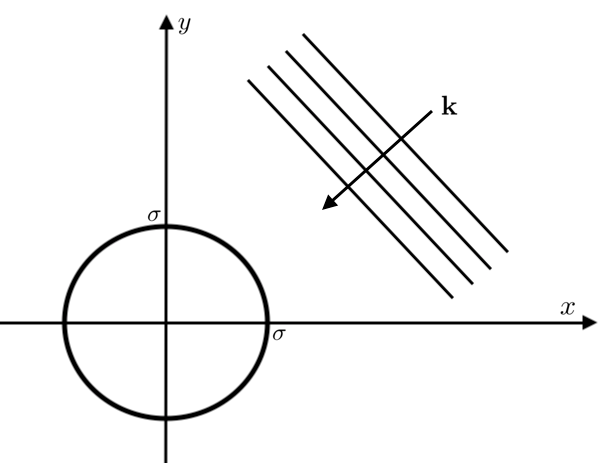
\includegraphics[width=6cm]{prob1/prob1_figures/sk_problem_1.png}
        \caption{Problem 1}
        \label{fig:problem_1}
    \end{figure}
%
Throughout this problem we will be concerned with finding an expression for the total velocity field around the cylinder, $\vec{u}$. As we showed in \ssref{ss:physical_interpretation}, it will be sufficient for us to seek $\Phi(x, y)$, since this is a 2D problem. \par
%
Let $\Phitot = \Phiin + \Phisc$, where $\Phiin$ is the incident field, and $\Phisc$ is the scattered field. All three of these must satisfy the Helmholtz equation.
%-----------------------------------------------------------------
%                   INCIDENT FIELD
%-----------------------------------------------------------------
\section{The incident field}
First let us consider $\Phiin$, the incident field. We choose Cartesian coordinates $(x,y)$, and polar coordinates $(r, \theta)$.
    \begin{propn}\label{propn:ch2_inc_field_intro}
    The incident field has the form
        \begin{equation}
            \Phiin = e^{-i(\vec{k}\cdot\vec{x})}
        \end{equation}
    \end{propn}
    \begin{proof}
    We need to show that this expression for $\Phiin$ satisfies the Helmholtz equation, \eqref{eq:helmholtz}. \par
        \begin{align*}
            \nabla^2 \Phiin
            &= \left[ \partialfrac{^2}{x^2} + \partialfrac{^2}{y^2} \right] e^{-i(\vec{k}\cdot\vec{x})} \\
            &= (-i)^2 a^2 e^{-i(ax+by)} + (-i)^2b^2 e^{-i(ax+by)}\\
            &= -(a^2+b^2)\Phiin
        \end{align*}
    Then,
        \begin{gather*}
            \nabla^2 \Phiin + k^2 \Phiin
            = -(a^2+b^2)\Phiin + k^2 \Phiin = 0\\
            \Rightarrow k^2-(a^2+b^2)=0
        \end{gather*}
    which is true by definition of the wave vector $\vec{k}$ (see definition \ref{defn:wave_vector}).
    \end{proof}
%
    \begin{propn}\label{propn:jacobi_expansion}
    \textbf{\emph{The Jacobi expansion.}}
        \[
        e ^{i \omega cos \varphi}
        = \sum^\infty_{n=-\infty} i^n J_n (\omega) e^{in\varphi}
        = \sum^\infty_{n=0} \epsilon_n i^n J_n(\omega) cos(n \varphi)
        \]
    where $\epsilon_n$ is the Neumann factor, defined as follows.
        \begin{align*}
            \epsilon_n =\left\{
                \begin{array}{c l}
                     1 & n = 0 \\
                     2 & n \geq 1
                \end{array}\right.
        \end{align*}
    \end{propn}
    \begin{proof} TBD \parencite[$\S$2.5]{martin06scattering}
    \end{proof}
%
    \begin{propn}\label{propn:ch2_inc_field_infty_sum}
    The incident field can be expressed as an infinite sum as follows.
        \begin{equation*}\label{eq:ch2_inc_field_infty_sum}
            \Phiin = \sum^{\infty}_{n=0} \epsilon_n i^n J_n(kr) \cos (n(\theta - \alpha))
        \end{equation*}
    \end{propn}
    \begin{proof}
    Follows directly from Propositions \ref{propn:ch2_inc_field_intro} and  \ref{propn:jacobi_expansion}.
    \end{proof}
%-----------------------------------------------------------------
%                       SCATTERED FIELD
%-----------------------------------------------------------------
\section{The scattered field}\label{ss:scattered_field}
We will now attempt to find an expression for the scattered field, $\Phisc$.
%-----------------------------------------------------------------
%                       separation of variables
%-----------------------------------------------------------------
\subsection{Separation of variables}\label{ss:ch2_sep_of_vars}
We don't want to make any assumptions about the form of the scattered field at this point, so we pose that it will depend on both $r$ and $theta$. We can hence employ the method of separation of variables once more:
    \begin{equation}
        \Phisc = R(r) \Theta(\theta).
    \end{equation}\par
%
Additionally, we know that $\Phisc$ must satisfy the Helmholtz equation:
    \begin{equation}\label{eq:phisc_helmholtz}
        \nabla^2 \Phisc + k^2 \Phisc = 0.
    \end{equation}
Hence,
    \begin{align*}
        \frac{1}{r} \partialfrac{}{r}
        \left( r \partialfrac{}{r} [R(r) \Theta(\theta)] \right)
        &+ \frac{1}{r^2} \partialfrac{^2}{\theta^2} [R(r) \Theta(\theta)]
        + k^2 R(r) \Theta(\theta) = 0 \\
        \Theta(\theta) \left( \frac{1}{r} \frac{dR(r)}{dr} + \frac{d^2 R(r)}{dr^2} \right)
        &+ \frac{R(r)}{r^2} \left( \frac{d^2 \Theta(\theta)}{d\theta^2}\right)
        + k^2 R(r) \Theta(\theta) = 0 \\
        \Theta ( \frac{1}{r} R' + R'')
        &+ \frac{1}{r^2} R \Theta'' + k^2 R \Theta = 0
    \end{align*}
    \begin{equation}
         \left ( r^2 \frac{R''}{R} + r\frac{R'}{R} + (kr)^2 \right ) = - \frac{\Theta''}{\Theta}
    \end{equation}\par
%
Let $\hat{\nu}$ be a constant. By the same argument as before (\ssref{ss:ch1_sep_of_vars}), we yield two ordinary differential equations:
    \begin{equation}\label{eq:ch2_theta_dep}
        \frac{d^2 \Theta}{d\theta^2} + \hat{\nu} \Theta = 0, ~\text{and}
    \end{equation}
    \begin{equation}\label{eq:ch2_r_dep}
        r^2 \frac{d^2 R}{dr^2} + r \frac{d R}{dr} + (k^2r^2 - \hat{\nu}) R = 0.
    \end{equation}
%
%------------------ theta dependence ----------------------------
\subsection{\texorpdfstring{$\theta$}{theta}-dependence}
To solve equation \eqref{eq:ch2_theta_dep} we need to consider three cases. \par
%
\textbf{Case 1.} Let $\hat{\nu} = 0$. This gives a linear solution:
    \begin{equation}
        \Theta(\theta) = A_1 \theta + B_1.
    \end{equation}\par
%
\textbf{Case 2.} Let $\hat{\nu} = \nu^2 > 0.$ Then we get an solution of exponential form.:
    \begin{equation}
        \Theta(\theta) = A_2 e^{\nu^2 \theta} + B_2 e^{- \nu^2 \theta}.
    \end{equation}\par
%
\textbf{Case 3.} Let $\hat{\nu}= - \nu^2 > 0$. This gives a solution of trigonometric form:
    \begin{equation}
        \Theta(\theta) = A_3 \cos(\nu\theta) + B_3 \sin(\nu\theta).
    \end{equation}\par
%
Since $\theta$ is the polar angular coordinate, we expect our solution to be $2\pi$ periodic. We can therefore discount Case 2. Case 1 is only periodic in the trivial case where $A_1 = 0$, and this is included in Case 3, when $A_3, B_3 = 0.$ We can therefore assume that $\hat{nu} = - \nu^2 > 0$.
%
\begin{propn} The general solution is
      \begin{equation}
          \Theta(\theta) = \sum^\infty_{n=0} C_n \cos(n (\theta - \alpha))
      \end{equation}
  \end{propn}
  \begin{proof} By Proposition \ref{propn:trig_sum_solution} we get a general solution of the form
      \begin{equation}
          \Theta(\theta) = \sum^\infty_{n=0} A_n \cos(\nu_n \theta) + B_n \sin(\nu_n \theta).
      \end{equation}
  Since $\Theta$ must be $2\pi$ periodic,
      \begin{align*}
          \Theta(\theta) &= \Theta(\theta + 2\pi).
      \end{align*}
  Hence we must have
      \begin{equation*}
          \cos(\nu_n \theta) = \cos(\nu_n \theta + \nu_n 2 \pi)
          ~\text{and}~
          \sin(\nu_n \theta) = \sin(\nu_n \theta + \nu_n 2 \pi)
          ~\text{for all}~ n \in \bb{Z}.
      \end{equation*}
      \begin{align*}
          \cos(\nu_n \theta) &= \cos(\nu_n \theta + \nu_n 2 \pi)\\
          &= \cos(\nu_n \theta) \cos(\nu_n 2 \pi) - \sin(\nu_n \theta) \sin(\nu_n 2 \pi) \text{ for all }\theta
      \end{align*}
      \begin{equation*}
          \cos(\nu_n 2 \pi) = 1
          \text{ and }
          \sin (\nu_n 2 \pi) = 0 \text{, so } \nu_n = n \in \bb{Z}
      \end{equation*}
  We can check that this works for the sine terms too:
      \begin{align*}
          \sin(\nu_n \theta + \nu_n 2\pi)
          &= \sin(n \theta + 2n \pi)\\
          &= \sin(n \theta) \cos(2n\pi) + \sin(2n\pi)\cos(n\theta)\\
          &= \sin(n\theta) = \sin(\nu_n \theta).
      \end{align*}
  This gives us a solution of the form
    \begin{equation*}
      \Theta(\theta) = \sum^\infty_{n=0} A_n \cos(n \theta) + B_n \sin(n \theta).
    \end{equation*}
  But we know that $\sin(n \theta) = 0 ~\forall n \in \bb{Z}, \theta \in \bb{R}$. We can therefore remove the second term, and also rewrite the first as follows:
    \begin{align*}
      A_n\cos(n\theta)
      &= \frac{A_n}{\sin(n\alpha)} [ \cos(n \theta) \cos(n \alpha) + \sin(n\theta)\sin(n\alpha)  ] \\
      &= C_n \cos(n(\theta - \alpha))
    \end{align*}
  Since for any given $n\in\bb{Z}$, $\sin(n\alpha)$ will be a constant.
  \end{proof}\par
%
%----------------------------------------------------------------
%                     r dependence
%----------------------------------------------------------------
\subsection{\texorpdfstring{$r$}{r}-dependence}
We now know that $\hat{\nu} = - \nu^2$, so we can rewrite \eqref{eq:ch2_r_dep} as follows:
    \begin{equation}\label{eq:ch2_r_dep_2}
        r^2 \frac{d^2 R}{dr^2} + r \frac{d R}{dr} + (k^2r^2 + \nu^2) R = 0.
    \end{equation}
    \begin{propn}
    Equation \eqref{eq:ch2_r_dep_2} is a Bessel differential equation of order $i\nu$.
    \end{propn}
    \begin{proof} Consider the substitution $r=kz$. Then
        \begin{align*}
            \frac{dR}{dr} = \frac{1}{k} \frac{dR}{dz}, ~~
            \frac{d^2R}{dr^2} = \frac{1}{k^2} \frac{d^2R}{dz^2}.
        \end{align*}\par
    %
    So \eqref{eq:ch2_r_dep_2} becomes
        \begin{align}
            \frac{r^2}{k^2}\frac{d^2R}{dz^2}
                + \frac{r}{k}\frac{dR}{dz}
                &+ (k^2r^2 + \nu^2)R = 0, \\
            z^2 \frac{d^2 R}{dz^2}
                + z \frac{dR}{dz}
                &+ (z^2 - (i\nu)^2)R = 0.
        \end{align}
    \end{proof}\par
%
Since $R(kr)$ satisfies a Bessel differential equation, the Bessel functions are solutions, and by the superposition principle any linear superposition of these is also a solution. We will need to consider the Sommerfeld radiation condition in order specify the general solution for $R(r)$. \par
%
  \begin{defn}\textbf{\emph{The Sommerfeld radiation condition.}} \label{defn:sommerfeld_radiation_condition}TBD
  \end{defn}
%
  \begin{propn}
      $\Phisc$ must satisfy the Sommerfeld radiation condition.
  \end{propn}
  \begin{proof} TBD
  \end{proof}
%
  \begin{propn}
      Hankel functions of the first kind satisfy the Sommerfeld radiation condition.
  \end{propn}
  \begin{proof}
      TBD, see \parencite[$\S$4.2]{martin06scattering}
  \end{proof}\par
%
From now on we refer to $H^{(1)}_\nu$ as $H_\nu$ for simplicity.
  \begin{propn}
    \[
    J_\nu(z) = (-1)^\nu J_\nu(z)
    \]
  \end{propn}
  \begin{proof}
    TBD
  \end{proof}
%
  \begin{propn}\label{propn:ch2_hankel_neg_identity}
    \[
    H_{-\nu}(z) = e^{i\nu \pi}H_\nu(z)
    \]
  \end{propn}
  \begin{proof}
    TBD
  \end{proof}
%
  \begin{propn}
    \begin{equation*}
      R(r) = \sum^\infty_{n=0} F_n H_n(kr) \text{, for $F_n$ constant.}
    \end{equation*}
  \end{propn}
  \begin{proof}
    From Proposition \ref{propn:ch2_hankel_neg_identity}
      \begin{align*}
        \sum^\infty_{n=-\infty} H_n(kr)
        & = \sum^\infty_{n=0} H_n(kr) + \sum^\infty_{n=0} e^{in\pi} H_n(kr)\\
        & = \sum^\infty_{n=0} F_n H_n(kr)
      \end{align*}
    since $e^{in\pi}$ is a constant for any given $n \in \bb{Z}.$
  \end{proof}
%----------------------------------------------------------------
%               General solution
%----------------------------------------------------------------
\subsection{General solution}
We can now combine our solutions for $\Theta$ and $R$ to find an expression for $\Phisc$.
%
    \begin{propn}
      The general solution for scattered field can be expressed as follows.
        \begin{equation} \label{eq:ch2_gen_eq_scattered_field}
            \Phisc = \sum^\infty_{n=-\infty} \epsilon_n i^n B_n H_n(kr) \cos(n(\theta-\alpha))
        \end{equation}
    \end{propn}
    \begin{proof} TBD. Need to show that:
      \[
      \Phisc = \sum^\infty_{n=-\infty} C_n H_n(kr) \cos(n(\theta-\alpha))
      \]
      with, $C_n = \epsilon_n i^n B_n$.
    \end{proof}
%----------------------------------------------------------------
%               Neumann boundary condition
%----------------------------------------------------------------
\subsection{Neumann boundary condition}\label{ss:ch2_neumann_bcs}
We first cosider the boundary at the cylinder wall to satisfy a Neumann boundary condition.
  \begin{defn}
    \parencite[$\S$1.3.2]{martin06scattering} A boundary is sound-hard if
      \begin{align*}
        \partialfrac{u}{r} = 0 \text{,  on } r = \sigma.
      \end{align*}
  \end{defn} \par
%
Equivalently, we can express this boundary condition in terms of $\Phi$:
  \begin{align*}
    \partialfrac{\Phi}{r}=0 \text{,  on } r = \sigma.
  \end{align*} \par
%
We can now apply this to find an expression for the constant terms in \eqref{eq:ch2_gen_eq_scattered_field}. Differentiating this equation gives
  \begin{equation}
    \sum^\infty_{n=0} \epsilon_n k i^n
    \{ J'_n(kr) + B_n H'_n(kr) \} \cos(n(\theta-\alpha)) = 0
  \end{equation}
Since $\cos(n(\theta - \alpha)) \neq 0 ~ \forall n, \theta$, it must be that the expression inside the braces must be zero for each $n$ at the boundary $r=\sigma$. Hence, we get an expression for $B_n$:
  \begin{equation}
    B_n= \frac{J'_n(k\sigma)}{H'_n(k\sigma)}.
  \end{equation}
%----------------------------------------------------------------
%               Dirichlet boundary condition
%----------------------------------------------------------------
\subsection{Dirichlet boundary condition}\label{ss:ch2_dirichlet_bcs}
We now consider the Dirichlet boundary condition.
  \begin{defn}
    \parencite[$\S$1.3.2]{martin06scattering} A body is sound-soft if
      \[
      u = 0 \text{,  on } r = \sigma
      \]
  \end{defn}
Hence, $\Phi_{sc} = - \Phi_{in}$ on $r=\sigma$,
  \begin{align*}
    \sum^\infty_{n=0} \epsilon_n i^n B_n H_n(kr) \cos(n((\theta-\alpha)))
    & = - \sum^\infty_{n=0} \epsilon_n i^n J_n(kr) \cos(n((\theta-\alpha))) \\
    \text{hence for all } n,~ B_n H_n (k\sigma) &= - J_n (k\sigma) \\
  \end{align*}
Hence the Dirichlet boundary condition specifies $B_n$ as follows.
  \begin{equation}
    B_n = \frac{- J_n(k\sigma)}{H_n(k\sigma)}
  \end{equation}
%----------------------------------------------------------------
%               TOTAL FIELD
%----------------------------------------------------------------
\section{Total field}
Throughout this chapter we have been searching for an expression for the resultant field of a plane wave with wave vector $\vec{k}$ incident on a cylinder radius $\sigma$, $\phi(x,y,z,t;\sigma, \vec{k})$.\par
%
    \begin{propn}
        \begin{equation*}
            \Phitot (r, \theta; \vec{k}, \sigma) =
            \sum^\infty_{n=0} \epsilon_n i^n \cos(n(\theta-\alpha))
             \{B_n H_n(kr) + J_n(kr)\}
        \end{equation*}
      where $B_n$ is specified by the boundary conditions outlined in \ssref{ss:ch2_dirichlet_bcs} and \ssref{ss:ch2_neumann_bcs}.
    \end{propn}
